\documentclass[hidelinks, a4paper,12pt, titlepage]{article}
\usepackage[a4paper,bottom = 0.58in,left = 1in,right = 1in,top = 1in]{geometry}
\usepackage{fontspec}
\usepackage{xunicode,xltxtra,url,parskip}
\usepackage{graphicx}
\usepackage{lipsum}% for auto generating text
\usepackage{afterpage}% for "\afterpage"
\usepackage{pagecolor}
\usepackage{hyperref}
\usepackage{sectsty}
\graphicspath{{screenshots/}}
\sectionfont{\fontsize{18}{24}\selectfont}
\setmainfont[Path=./fonts/,BoldFont = Lato-Bold.ttf,ItalicFont = Lato-LightItalic.ttf]{Lato-Light.ttf}
\usepackage[usenames,dvipsnames]{xcolor}
\begin{document}
\newpagecolor{black}\afterpage{\restorepagecolor}
\vspace{0pt}
{\center 
\includegraphics[scale=0.44]{logo.png}}
\vspace{20pt}
{\center \color{white} \fontsize{50}{60}\selectfont USER \\DOCUMENTATION\\}
\setmainfont[Path=./fonts/,BoldFont = Lato-Bold.ttf,ItalicFont = Lato-Italic.ttf]{Lato-Regular.ttf}

\vspace{90pt}
{\center \color{white} \fontsize{20}{22}\selectfont TEAM ECLIPSE\\}
\vspace{10pt}
\setmainfont[Path=./fonts/,BoldFont = Lato-Bold.ttf,ItalicFont = Lato-LightItalic.ttf]{Lato-Light.ttf}
{\center \color{white} \fontsize{15}{18}\selectfont October 29,\, 2017\\}
\setmainfont[Path=./fonts/,BoldFont = Lato-Bold.ttf,ItalicFont = Lato-Italic.ttf]{Lato-Regular.ttf}
\vspace{75pt}
{\center \color{white} \fontsize{15}{18}\selectfont Vighnesh Reddy Konda\hfill|\hfill Naman Jain\hfill|\hfill Satti Vamsi Krishna Reddy\\}
 \newpage
{ \renewcommand{\baselinestretch}{1.5} 
\tableofcontents
}
 \newpage
\section{Homepage}
\textbf{URL:} \texttt{/}

As soon as you login you get this screen where you can login if you are already a registered user else sign up
\begin{center}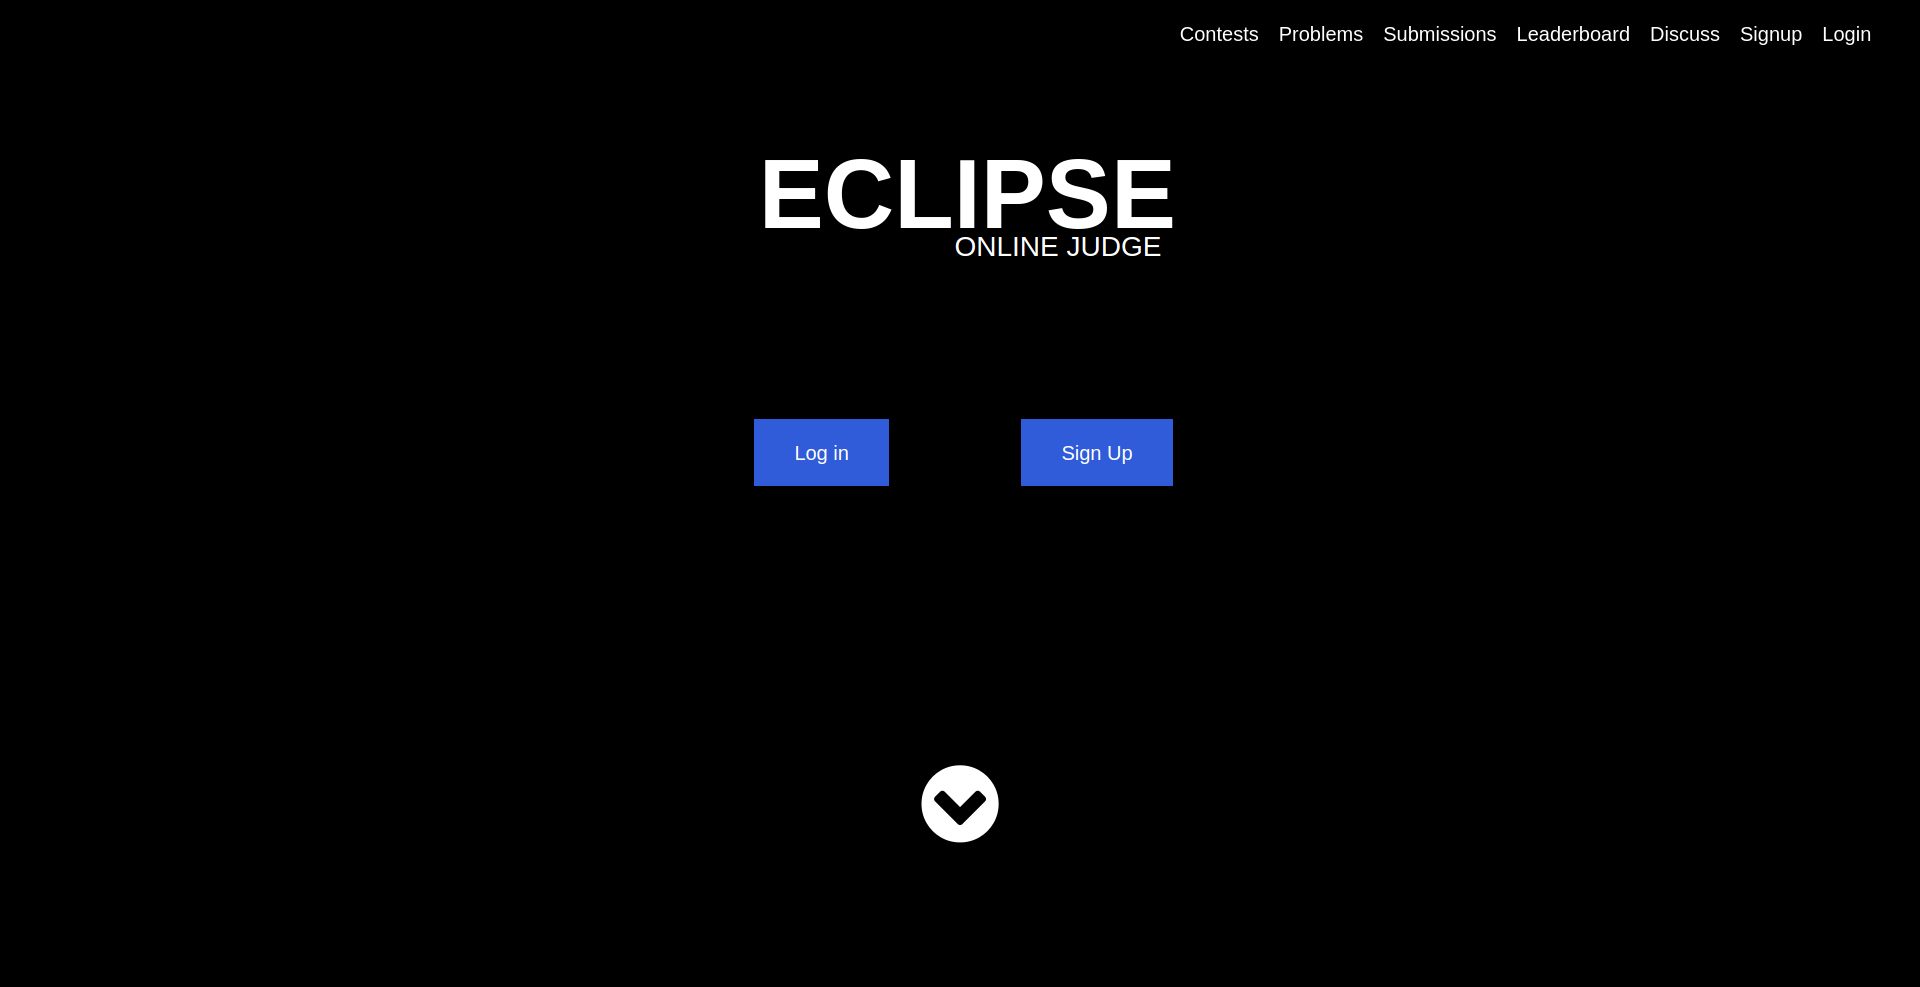
\includegraphics[width=0.9\textwidth]{Homepage.png}\end{center}


 
\section{Sign Up}
\textbf{URL:} \texttt{/signup}

This is the place where you can register for EclipseOJ
\begin{center}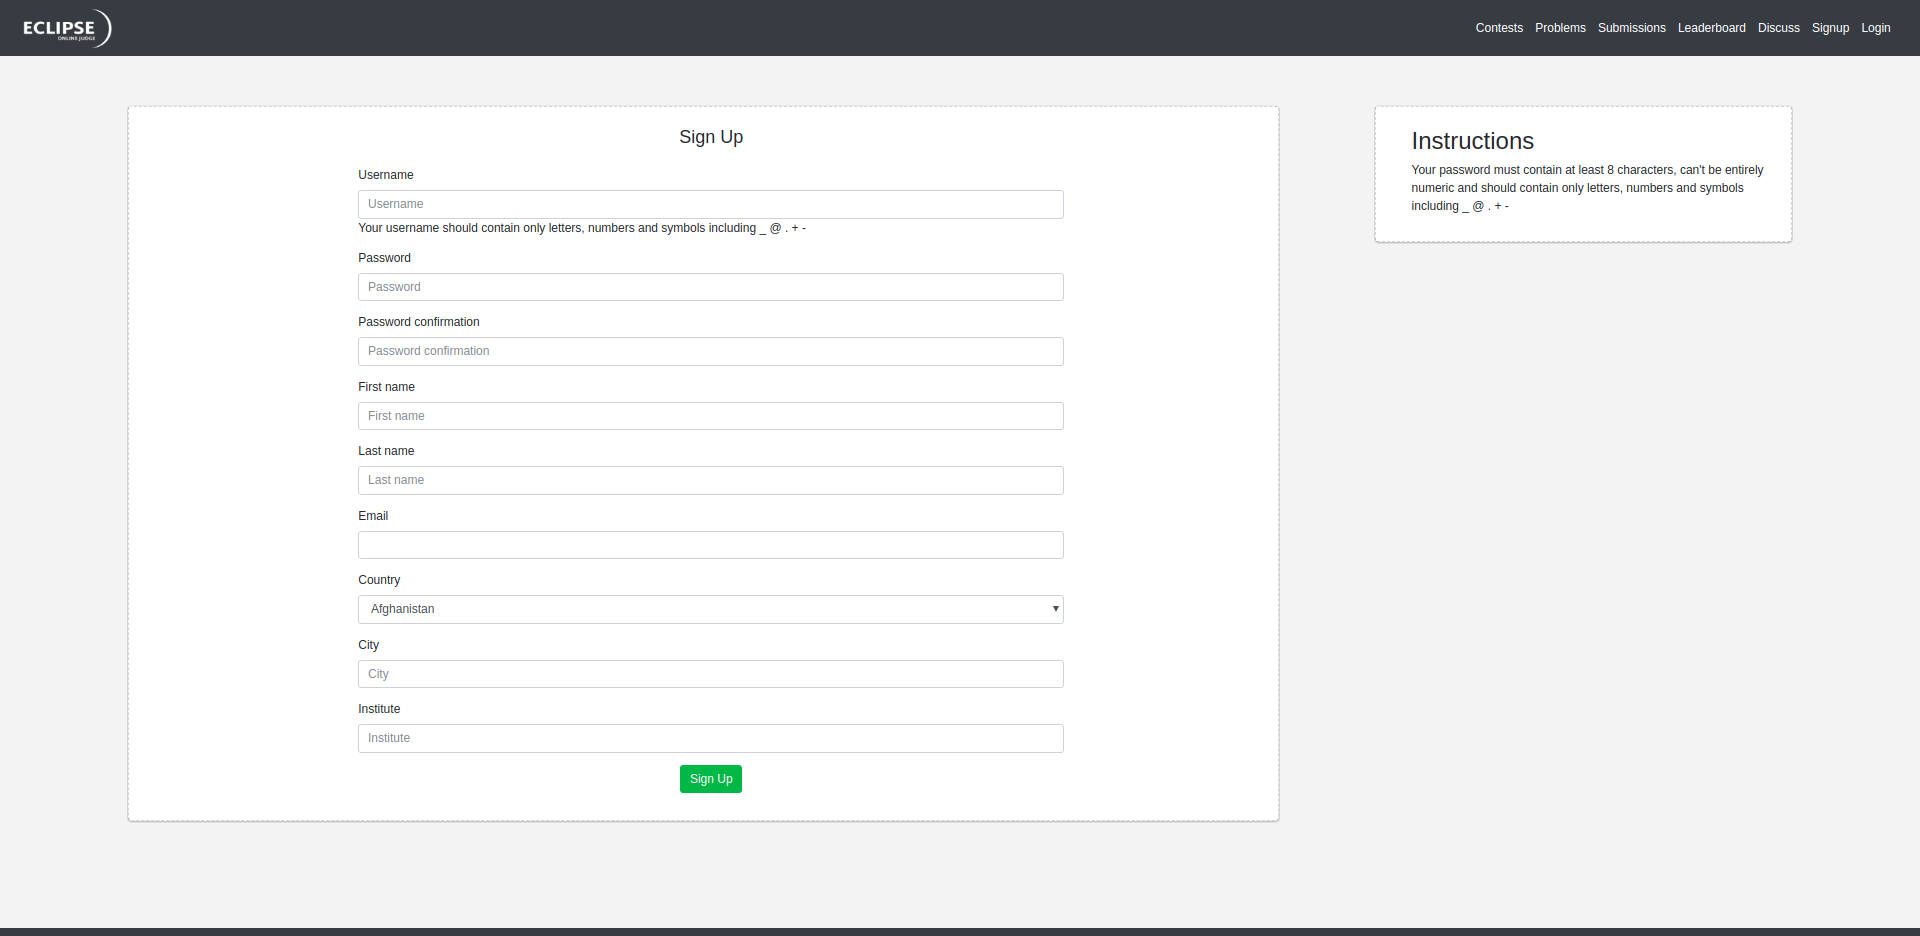
\includegraphics[width=0.9\textwidth]{Signup.png}\end{center}

\newpage
 
\section{Contests}
\subsection{All contests}
\textbf{URL:} \texttt{/contests}

This is the place where you can find the links to all the contests
\begin{center}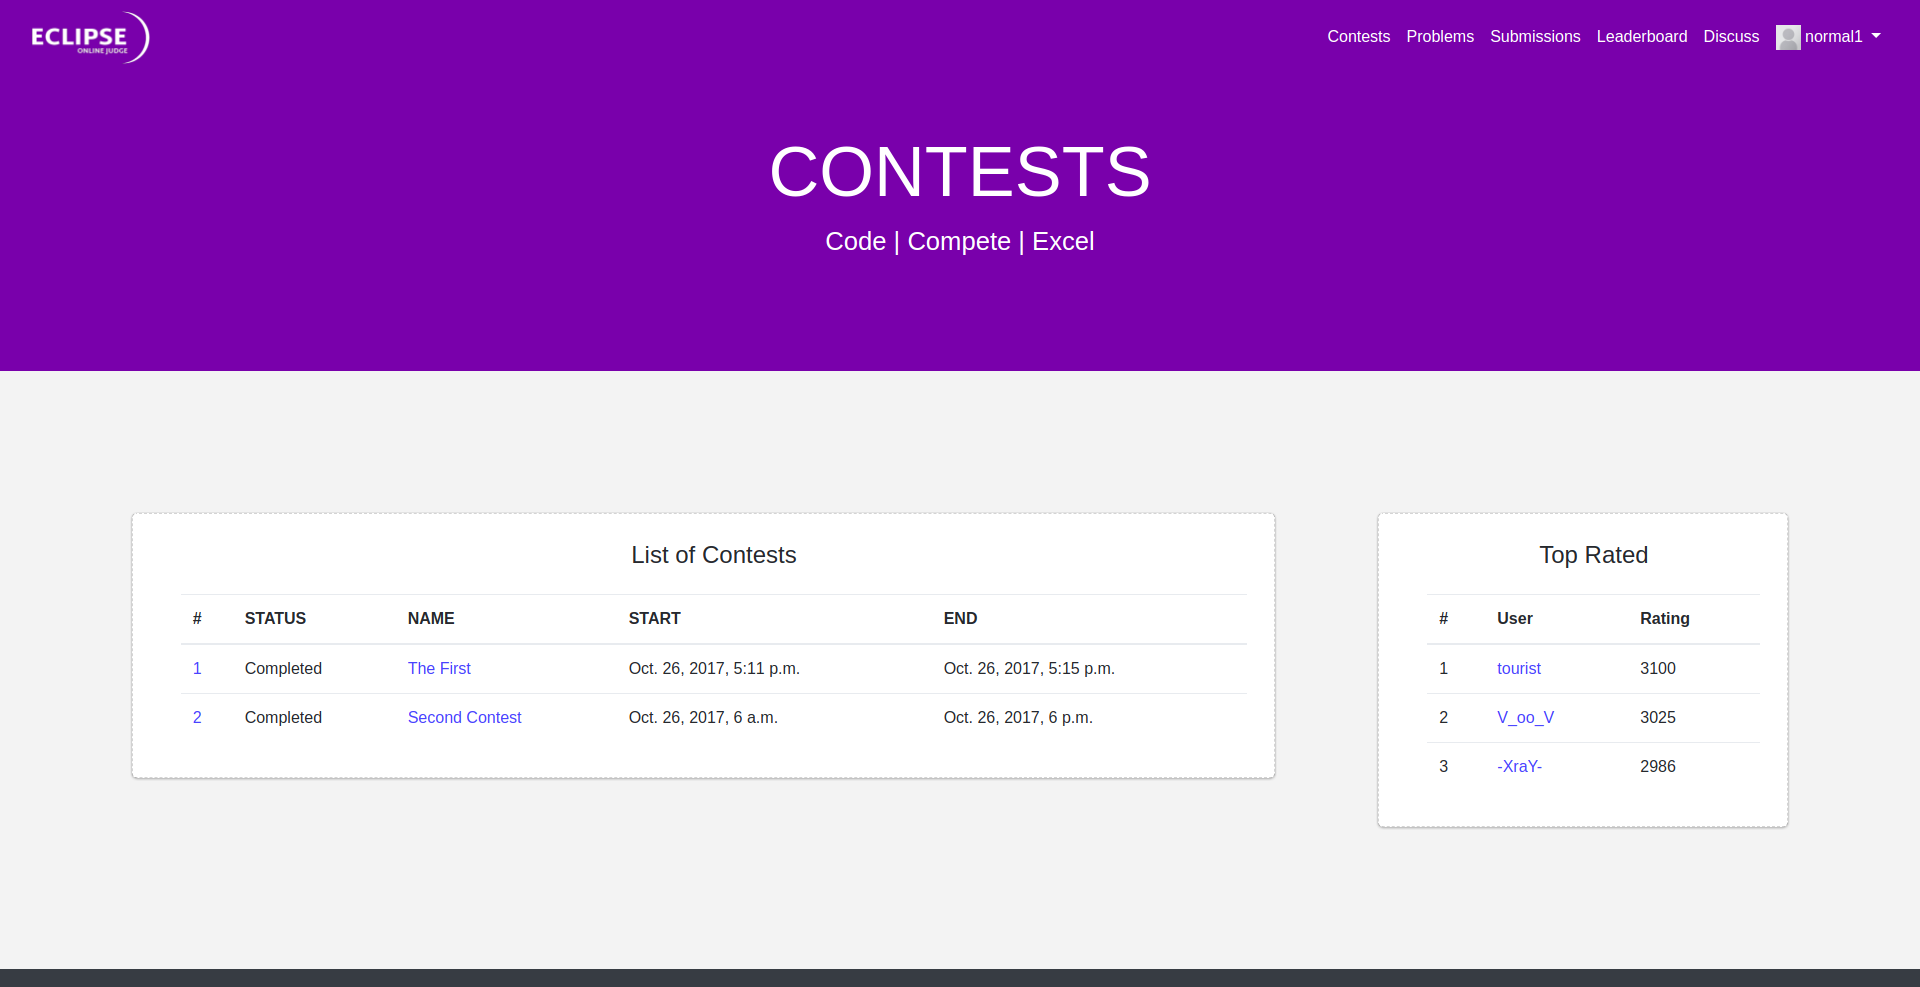
\includegraphics[width=0.9\textwidth]{contests.png}\end{center}

We also display the status of the contests like Ongoing, Completed and Future

The right panel shows the top 5 users  
 
\subsection{Specific Contest}
\textbf{URL:} \texttt{/contests/contestID}

This is the place where you can get all the links to the problems of this contest if it is in the past or running currently
\begin{center}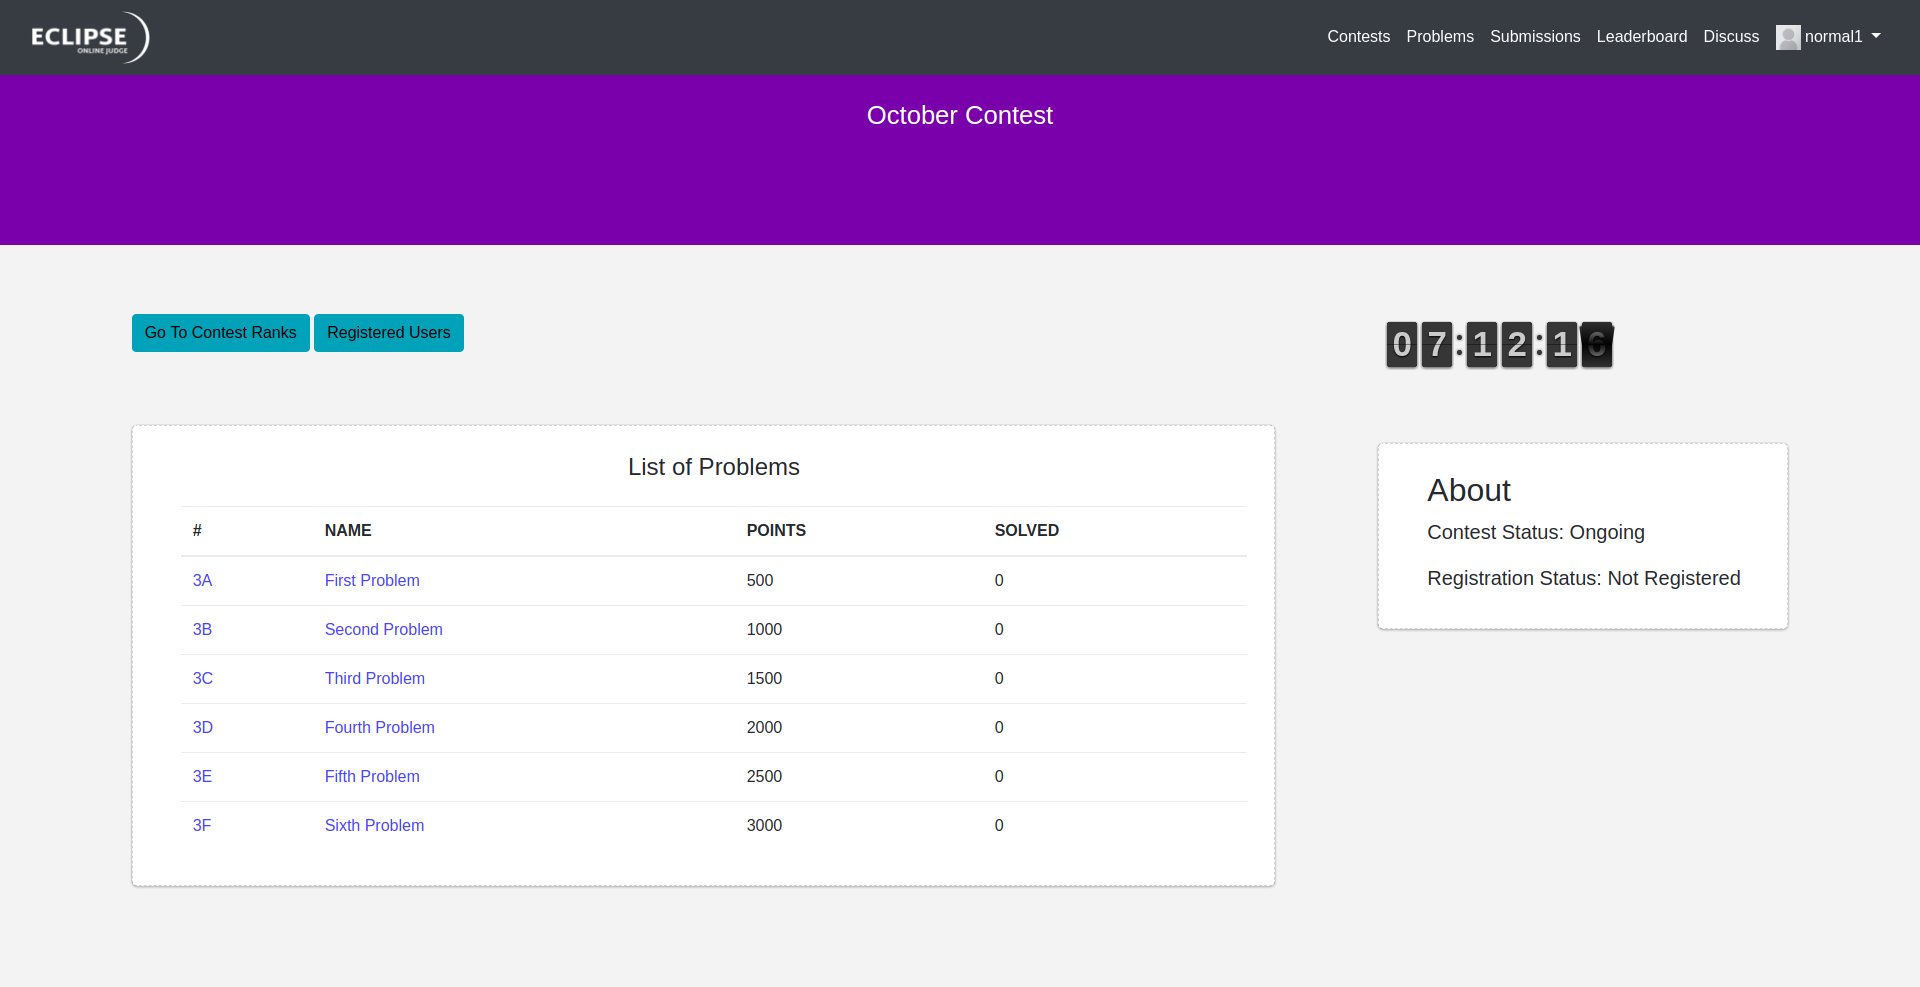
\includegraphics[width=0.9\textwidth]{runningcontest.png}\end{center}
 
\newpage

\section{Problems}
\subsection{All Problems}
\textbf{URL:} \texttt{/problems}

Contains a list of all problems
\begin{center}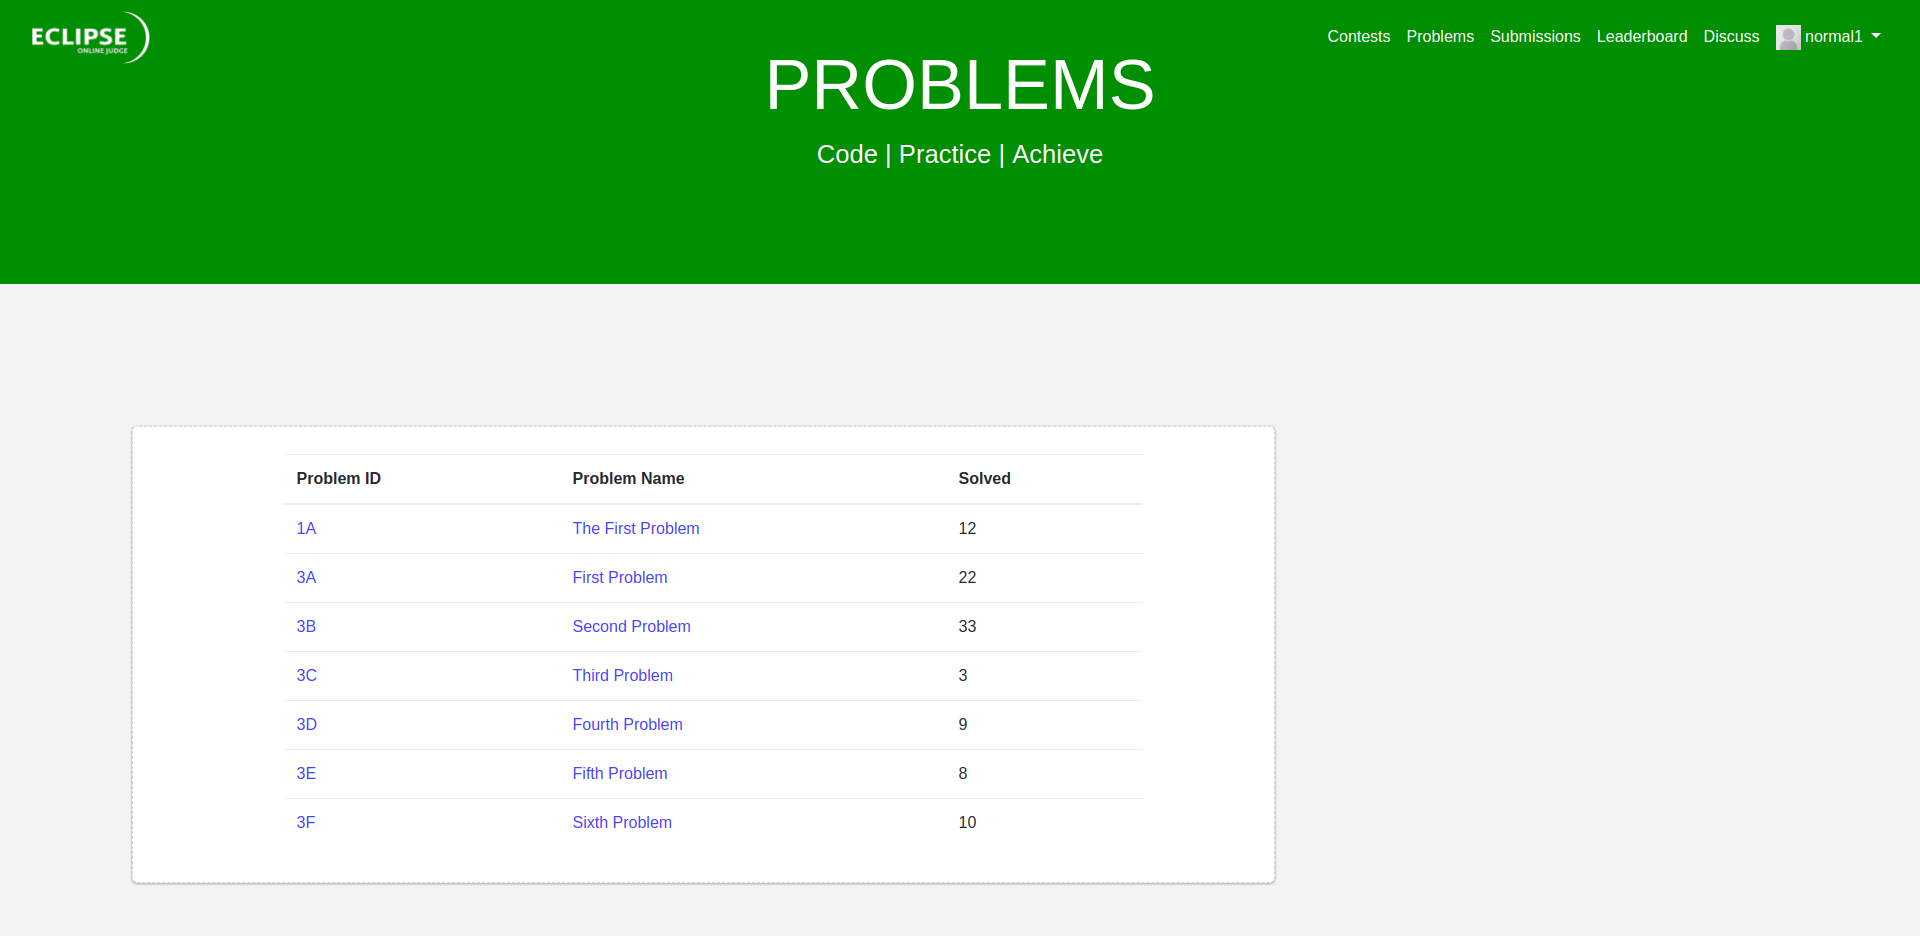
\includegraphics[width=0.9\textwidth]{allproblems.png}\end{center}
 
\subsection{Specific Problem}
\textbf{URL:} \texttt{/problems/problemID}

This is the place where you see the problem statement and submission format
\begin{center}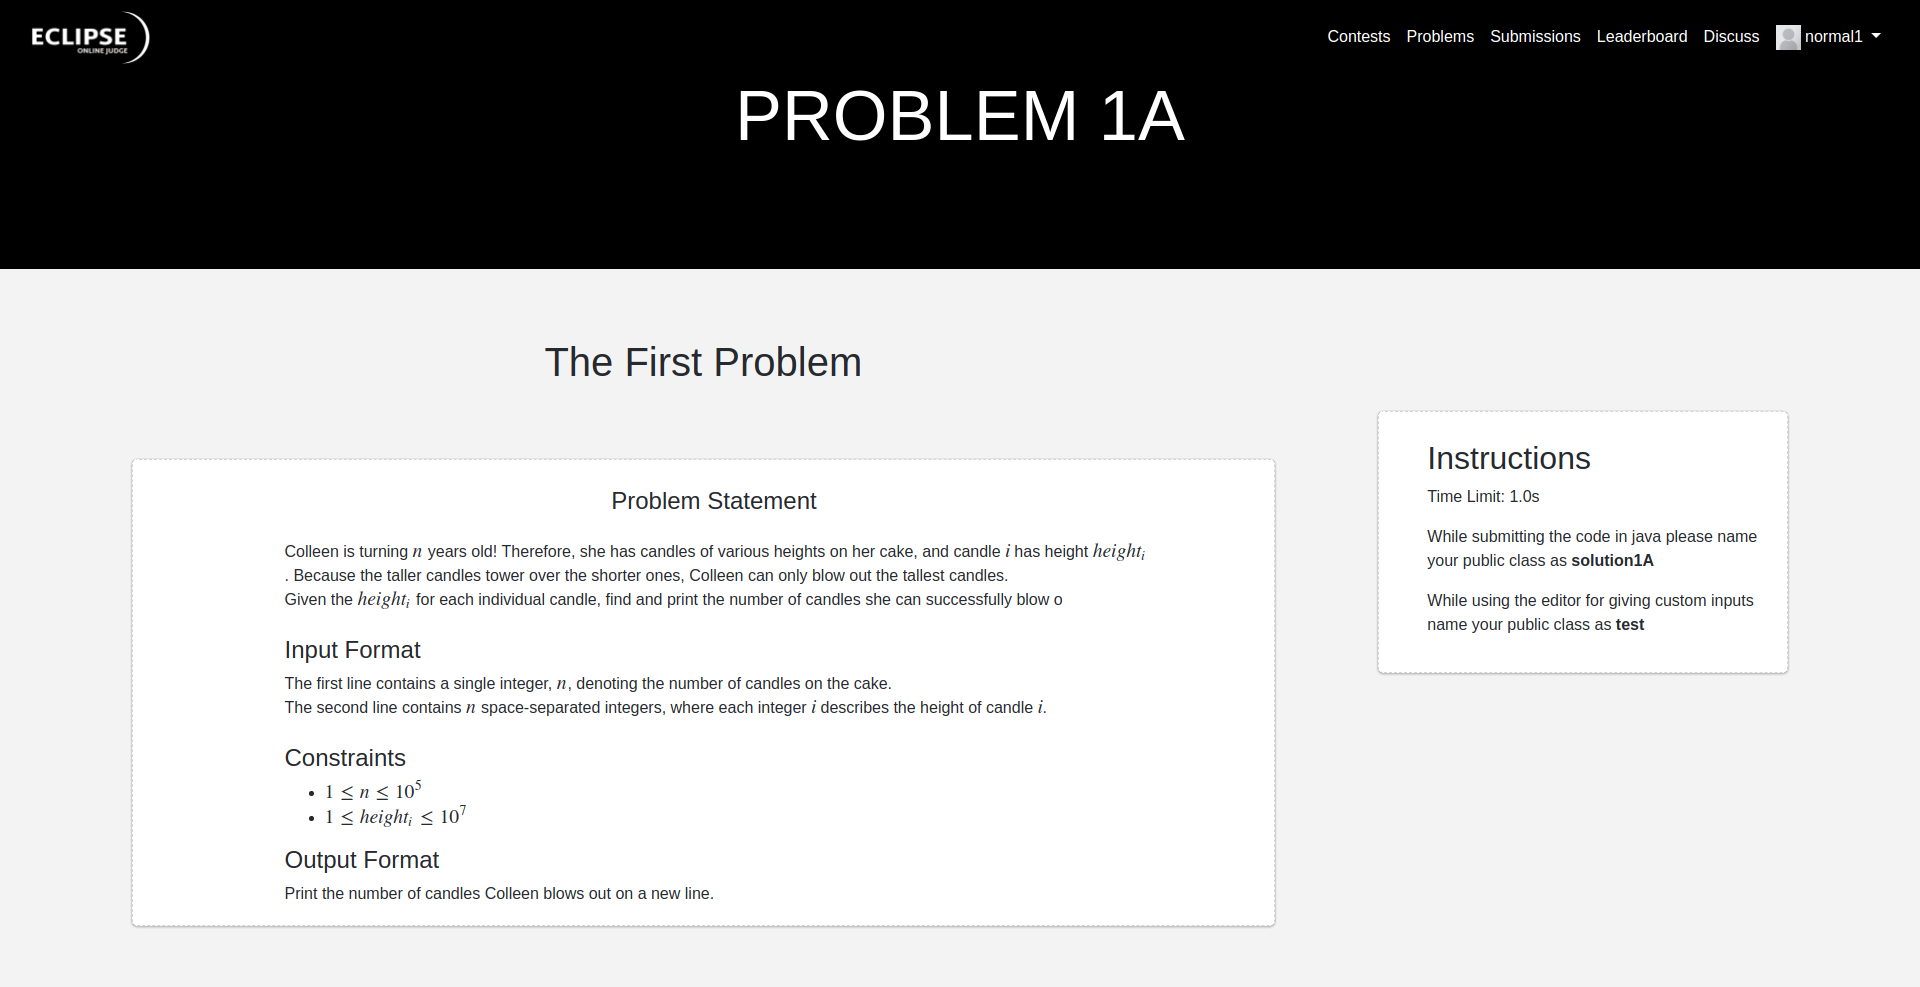
\includegraphics[width=0.9\textwidth]{problemstatement.png}\end{center}
 
 \newpage

\section{Text Editor}
This is the place where you can code online and check with your custom inputs and can submit directly 
You will get the editor below every problem where you can code in 5 languages. The editor is customizable with support for a dark and a light theme
\begin{center}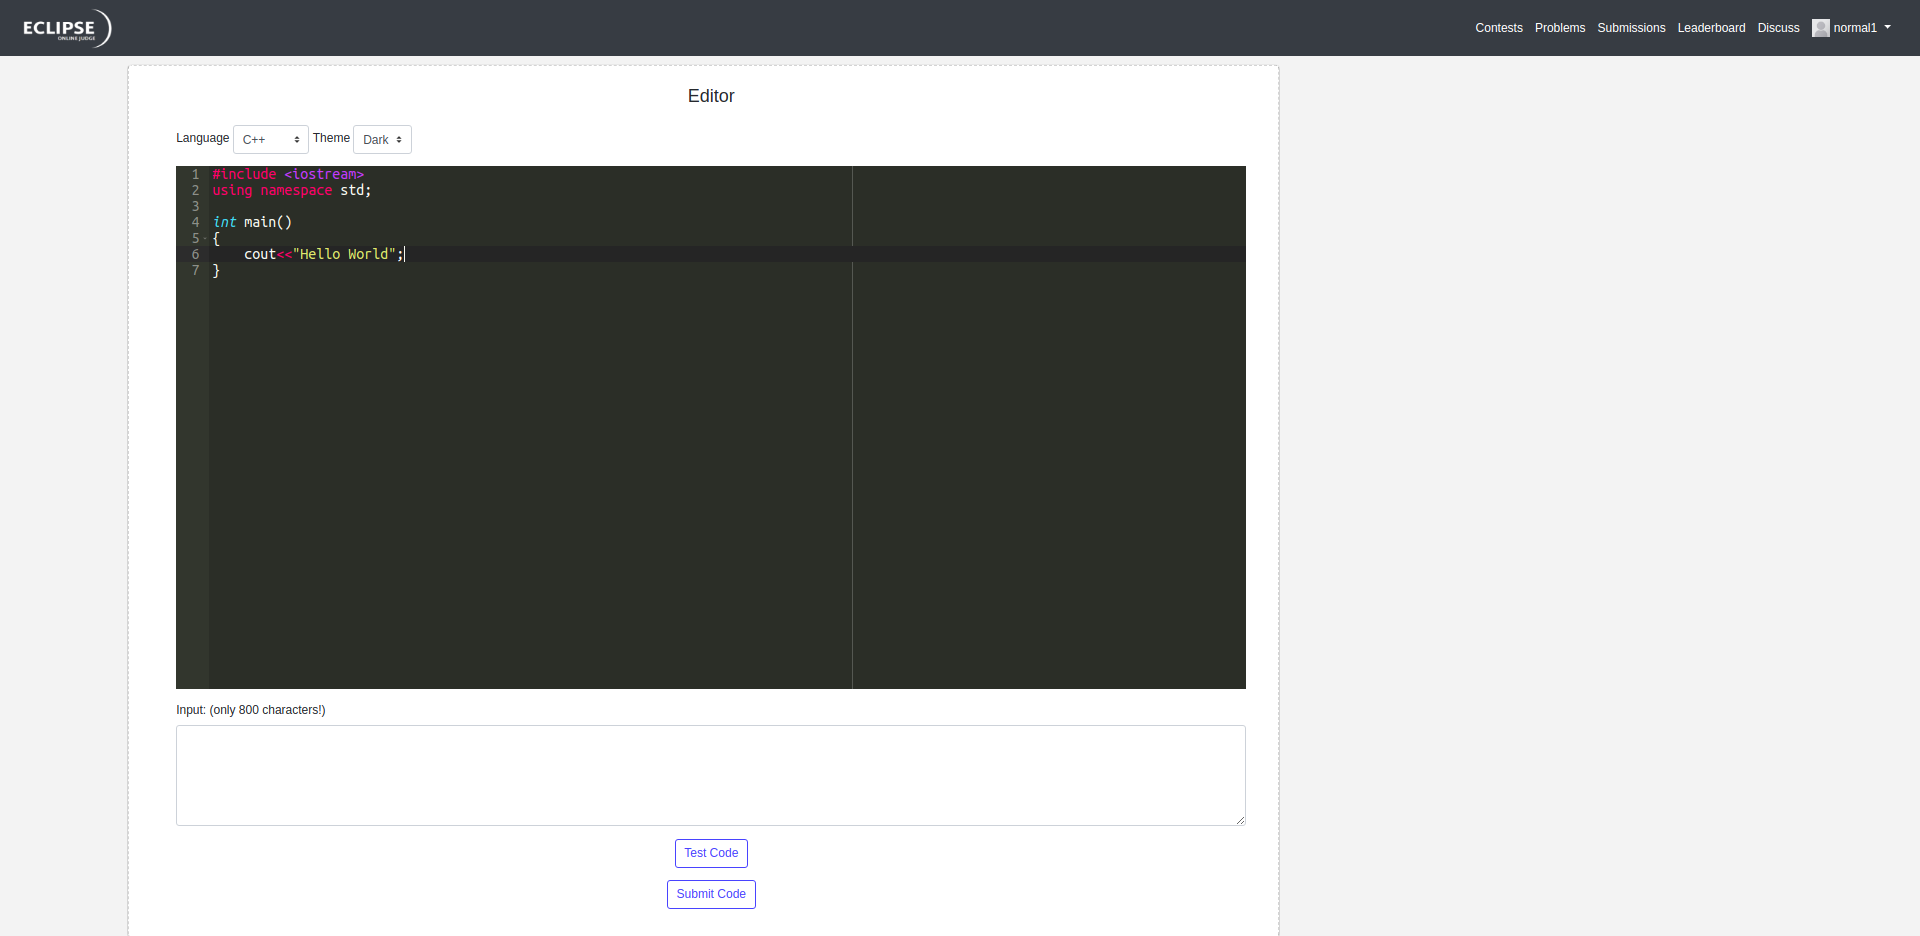
\includegraphics[width=0.9\textwidth]{texteditor.png}\end{center}
 
\section{Leaderboard}
\textbf{URL:} \texttt{/leaderboard}

This is the place where you can see the all the users with their ratings in decreasing order i.e; Highest rating first
You can also search for any class of users according to their Institution, Country, City etc
\begin{center}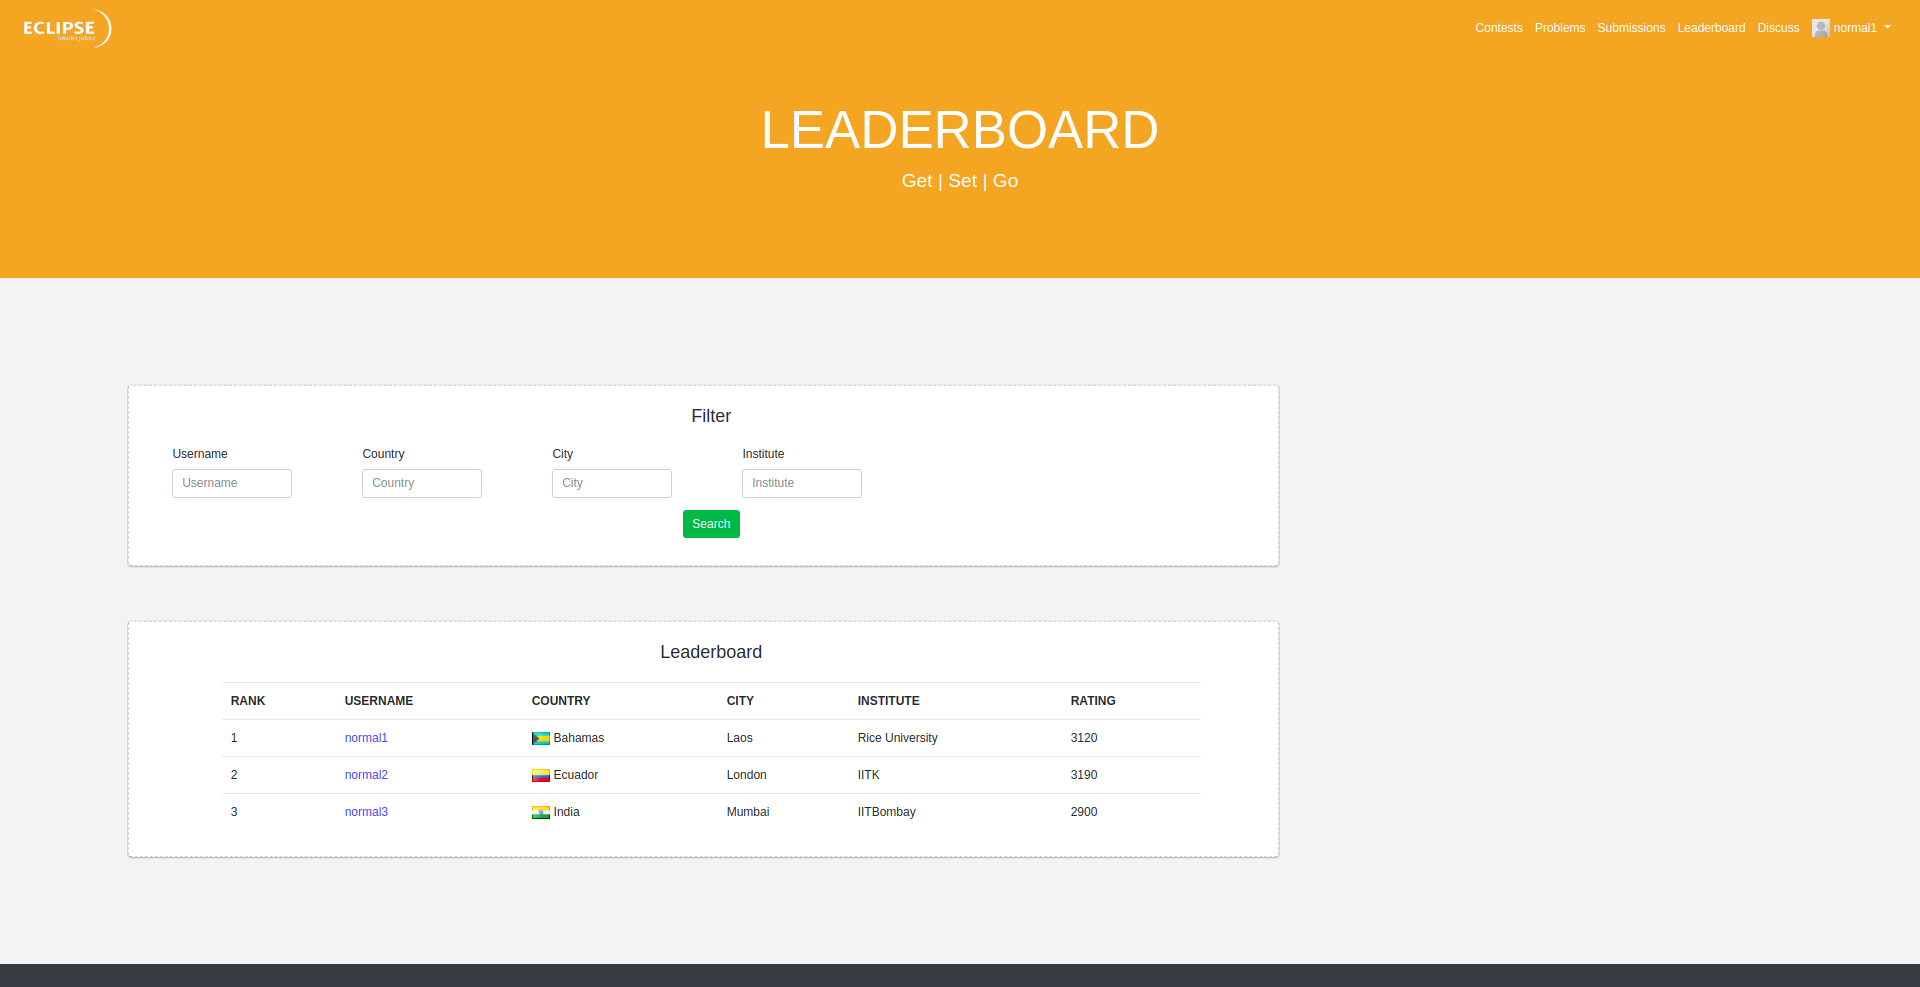
\includegraphics[width=0.9\textwidth]{leaderboard.png}\end{center} 
 
\newpage

\section{Discussion Forum}
\textbf{URL:} \texttt{/discuss}

This is the place people can post their doubts or answer already posted doubts
\begin{center}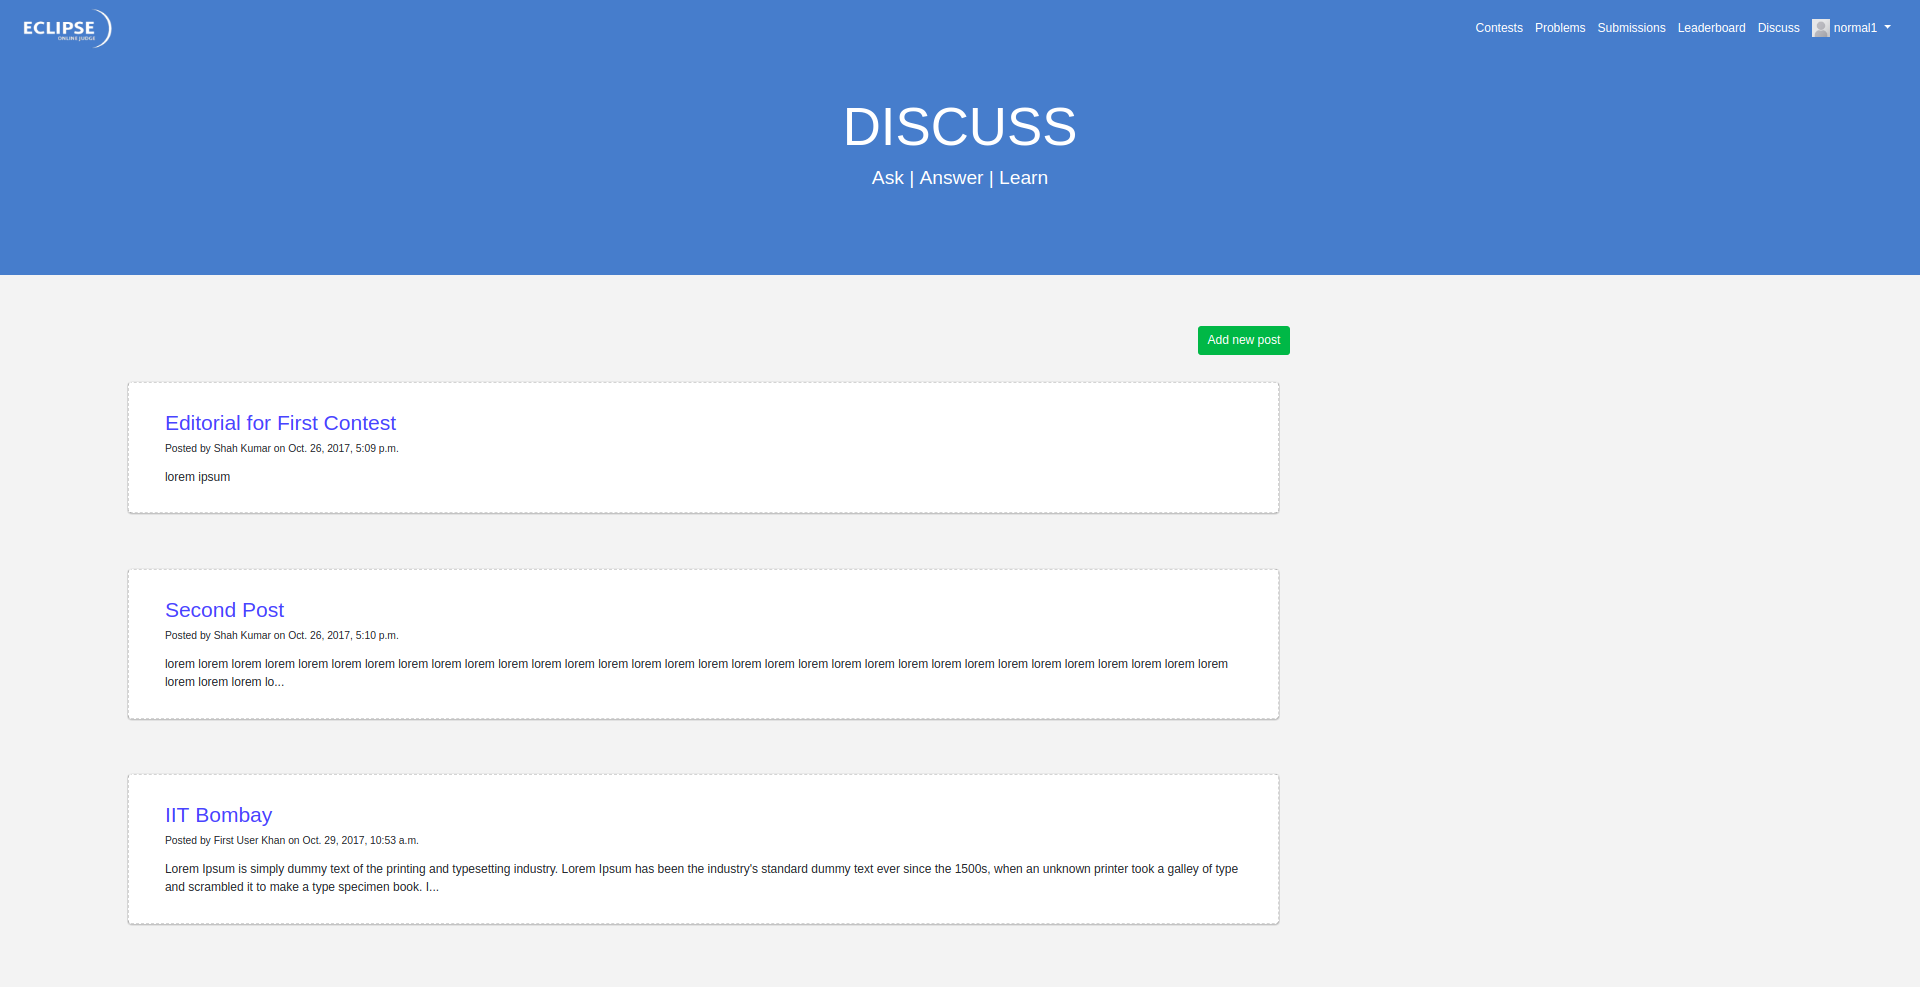
\includegraphics[width=0.84\textwidth]{Discuss.png}\end{center} 


\section{Submissions}
\textbf{URL:} \texttt{/submissions}

This is the place where you can see all the submissions with their verdicts
\begin{center}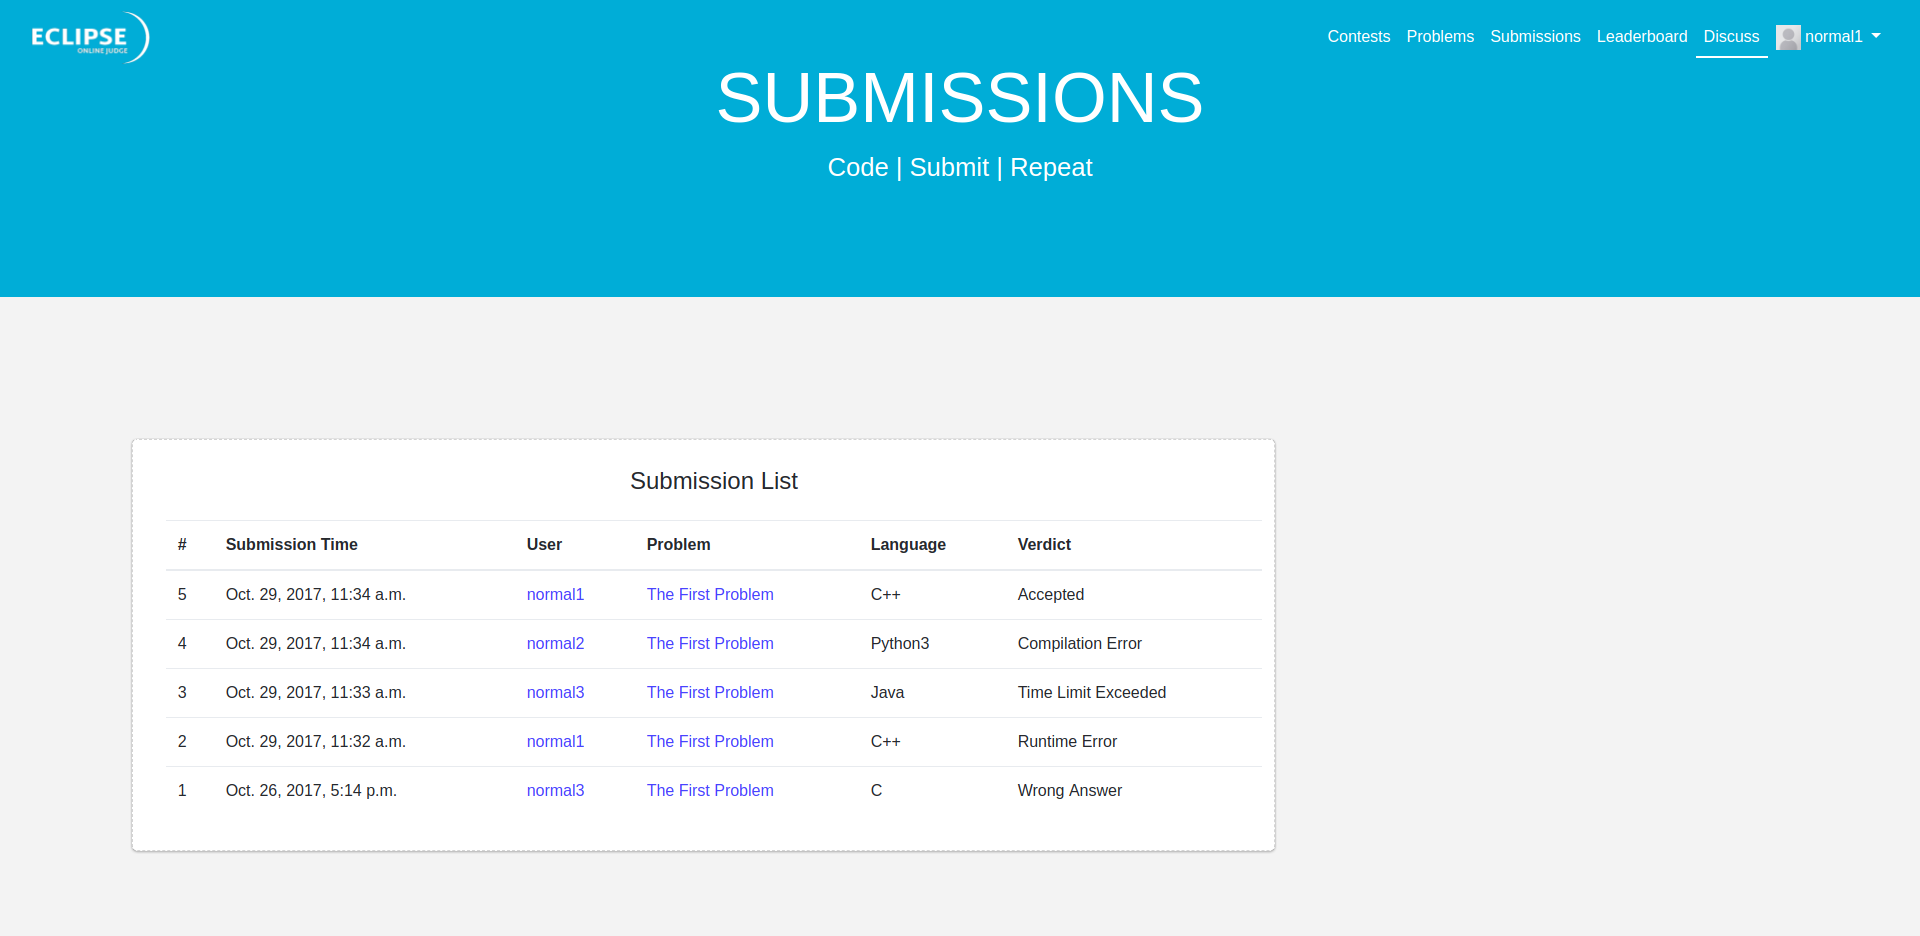
\includegraphics[width=0.84\textwidth]{submissions.png}\end{center} 
 

\section{Rating System}
Our rating system is similiar to Elo Based rating system. If player A has rating $R_A$ and player B has rating $R_B$ then the expected score for player A is $$E_A = \frac{1}{1+10^{(R_B-R_A)/400}}$$

\end{document}